% Compile with Tectonic:
%   conda run -n alphagenome tectonic docs/rna_seq11_group_meeting_20260518.tex
% Or with XeLaTeX on a machine with a CJK LaTeX distribution.
\documentclass[UTF8,aspectratio=169,10pt]{ctexbeamer}

\usetheme{Boadilla}
\usecolortheme{dolphin}
\setbeamertemplate{navigation symbols}{}
\setbeamertemplate{footline}[frame number]

\usepackage{booktabs}
\usepackage{graphicx}
\usepackage{tikz}
\usepackage{pgfplots}
\usetikzlibrary{arrows.meta,positioning}
\pgfplotsset{compat=1.18}

\definecolor{agblue}{RGB}{38,88,156}
\definecolor{aggreen}{RGB}{37,125,97}
\definecolor{agred}{RGB}{174,74,65}
\definecolor{aggray}{RGB}{92,102,112}

\setbeamercolor{title}{fg=agblue}
\setbeamercolor{frametitle}{fg=agblue}
\setbeamercolor{structure}{fg=agblue}

\title[C. elegans RNA-seq Adapter]{C. elegans 11-track RNA-seq\\AlphaGenome Adapter Experiments}
\subtitle{Frozen trunk adaptation, baselines, and follow-up pilots}
\author{Ziyang Huang}
\date{2026-05-18}

\newcommand{\smallnote}[1]{\vspace{0.4em}{\scriptsize\color{aggray}#1}}

\begin{document}

\begin{frame}
  \titlepage
\end{frame}

\begin{frame}{数据与划分}
  \begin{columns}[T,onlytextwidth]
    \begin{column}{0.45\textwidth}
      \begin{itemize}
        \item Reference：C. elegans WBcel235
        \item 20 个 sample-level RNA-seq bigWig
        \item 整理为 11 个 grouped RNA-seq tracks
        \item window：1,048,576 bp
        \item stride：524,288 bp
        \item target：clip negative + log1p
      \end{itemize}
    \end{column}
    \begin{column}{0.51\textwidth}
      \centering
      \begin{tabular}{lcc}
        \toprule
        Split & Chromosome & NPZ \\
        \midrule
        Train & I--IV & 116 \\
        Valid & V & 39 \\
        Test & X & 33 \\
        \bottomrule
      \end{tabular}

      \smallnote{MtDNA excluded; chromosome holdout.}

      \vspace{0.8em}
      \begin{tabular}{ll}
        \toprule
        Tensor & Shape \\
        \midrule
        DNA input & $[B,4,1048576]$ \\
        RNA-seq target & $[B,11,1048576]$ \\
        mask & $[B,11,1]$ \\
        \bottomrule
      \end{tabular}
    \end{column}
  \end{columns}
\end{frame}

\begin{frame}{模型结构}
  \centering
  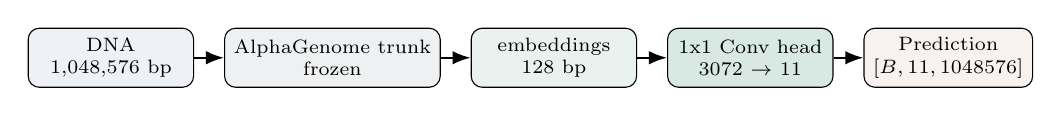
\begin{tikzpicture}[
    font=\scriptsize,
    node distance=0.38cm,
    block/.style={draw,rounded corners,align=center,minimum height=0.75cm,minimum width=2.10cm},
    arrow/.style={-{Latex[length=2.3mm]},thick}
  ]
    \node[block,fill=agblue!8] (dna) {DNA\\1,048,576 bp};
    \node[block,fill=aggray!10,right=of dna] (trunk) {AlphaGenome trunk\\frozen};
    \node[block,fill=aggreen!10,right=of trunk] (emb) {embeddings\\128 bp};
    \node[block,fill=aggreen!18,right=of emb] (head) {1x1 Conv head\\3072 $\rightarrow$ 11};
    \node[block,fill=agred!8,right=of head] (out) {Prediction\\$[B,11,1048576]$};
    \draw[arrow] (dna) -- (trunk);
    \draw[arrow] (trunk) -- (emb);
    \draw[arrow] (emb) -- (head);
    \draw[arrow] (head) -- (out);
  \end{tikzpicture}

  \smallnote{Head output is on the 128 bp grid, then linearly interpolated to 1,048,576 target positions.}

  \vspace{1.1em}
  \begin{columns}[T,onlytextwidth]
    \begin{column}{0.48\textwidth}
      \begin{block}{Trainable}
        adapter head：\textbf{33,803} parameters
      \end{block}
    \end{column}
    \begin{column}{0.48\textwidth}
      \begin{block}{Frozen}
        AlphaGenome trunk：\textbf{450,452,613} parameters
      \end{block}
    \end{column}
  \end{columns}
\end{frame}

\begin{frame}{主结果：valid MSE}
  \centering
  \begin{tikzpicture}
    \begin{axis}[
      width=0.95\textwidth,
      height=0.62\textheight,
      ybar,
      ymin=0.9,
      ymax=1.82,
      ylabel={Valid MSE},
      symbolic x coords={Mean,Tiny h64,128bp 500,128bp 5000,1bp DDP,LoRA-A,LoRA-B},
      xtick=data,
      x tick label style={rotate=0,anchor=north,align=center,font=\scriptsize,text width=1.35cm},
      bar width=13pt,
      nodes near coords,
      nodes near coords style={font=\tiny,rotate=0,anchor=south,yshift=1pt},
      every node near coord/.append style={
        /pgf/number format/fixed,
        /pgf/number format/precision=2
      },
      every axis plot/.append style={fill=agblue!25,draw=agblue!45}
    ]
      \addplot coordinates {
        (Mean,1.7282558)
        (Tiny h64,1.553865)
        (128bp 500,1.2418628)
        (128bp 5000,1.0609935)
        (1bp DDP,1.4771859)
        (LoRA-A,1.0613562)
        (LoRA-B,1.067338)
      };
    \end{axis}
  \end{tikzpicture}

  \smallnote{模型选择只看 valid。test 只在最终 selected checkpoint 上评估一次。}
\end{frame}

\begin{frame}{128 bp adapter 训练曲线}
  \centering
  \begin{tikzpicture}
    \begin{axis}[
      width=0.93\textwidth,
      height=0.62\textheight,
      xlabel={Step},
      ylabel={Valid MSE},
      ymin=1.03,
      ymax=1.46,
      xmin=0,
      xmax=5100,
      grid=both,
      grid style={draw=gray!18},
      legend style={at={(0.98,0.98)},anchor=north east,font=\scriptsize}
    ]
      \addplot[color=agblue,mark=*,thick] coordinates {
        (250,1.4321554) (500,1.2141448) (750,1.1533484)
        (1000,1.1391212) (1250,1.1607189) (1500,1.1319546)
        (1750,1.1639107) (2000,1.1181387) (2250,1.1082077)
        (2500,1.0989698) (2750,1.0882852) (3000,1.0935162)
        (3250,1.0837174) (3500,1.1061893) (3750,1.0840694)
        (4000,1.0615692) (4250,1.0609935) (4500,1.0840007)
        (4750,1.0764805) (5000,1.1053824)
      };
      \addlegendentry{128 bp adapter}
      \addplot[color=agred,dashed,thick] coordinates {(4250,1.03) (4250,1.46)};
      \addlegendentry{selected step 4250}
    \end{axis}
  \end{tikzpicture}
\end{frame}

\begin{frame}{valid/test 总体指标}
  \centering
  \begin{tabular}{lccc}
    \toprule
    Split & MSE & MAE & Pearson \\
    \midrule
    Valid & \textbf{1.0609935} & \textbf{0.71866247} & \textbf{0.58809888} \\
    Test & 1.1711332 & 0.76486897 & 0.55539986 \\
    \bottomrule
  \end{tabular}

  \vspace{1.1em}
  \begin{block}{解释}
    Test 与 valid 指标接近，跨染色体泛化表现稳定。
  \end{block}
\end{frame}

\begin{frame}{per-track Pearson}
  \centering
  \begin{tikzpicture}
    \begin{axis}[
      width=0.94\textwidth,
      height=0.62\textheight,
      xlabel={Track index},
      ylabel={Pearson},
      ymin=0.48,
      ymax=0.67,
      xmin=-0.5,
      xmax=10.5,
      xtick={0,1,2,3,4,5,6,7,8,9,10},
      grid=both,
      grid style={draw=gray!18},
      legend style={at={(0.02,0.98)},anchor=north west,font=\scriptsize}
    ]
      \addplot[color=agblue,mark=*,thick] coordinates {
        (0,0.54028078) (1,0.54484031) (2,0.55136293)
        (3,0.54676353) (4,0.57354249) (5,0.60321)
        (6,0.60869882) (7,0.61981902) (8,0.63397316)
        (9,0.64370303) (10,0.58150481)
      };
      \addlegendentry{Valid}
      \addplot[color=agred,mark=square*,thick] coordinates {
        (0,0.51305557) (1,0.51497802) (2,0.53053846)
        (3,0.53190608) (4,0.55922813) (5,0.53393285)
        (6,0.55428168) (7,0.57475091) (8,0.59417222)
        (9,0.59174095) (10,0.54218363)
      };
      \addlegendentry{Test}
    \end{axis}
  \end{tikzpicture}

  \smallnote{Muscle tracks generally show higher Pearson than intestine tracks in this split.}
\end{frame}

\begin{frame}{1 bp 与 LoRA：可行但未提升}
  \begin{columns}[T,onlytextwidth]
    \begin{column}{0.48\textwidth}
      \centering
      \begin{tikzpicture}
        \begin{axis}[
          width=\textwidth,
          height=0.54\textheight,
          ybar,
          ymin=1.03,
          ymax=1.55,
          ylabel={Best valid MSE},
          symbolic x coords={128bp,1bp,LoRA-A,LoRA-B},
          xtick=data,
          x tick label style={font=\scriptsize},
          bar width=14pt,
          nodes near coords,
          nodes near coords style={font=\tiny,rotate=90,anchor=west}
        ]
          \addplot[fill=aggreen!65,draw=aggreen!90] coordinates {
            (128bp,1.0609935)
            (1bp,1.4771859)
            (LoRA-A,1.0613562)
            (LoRA-B,1.067338)
          };
        \end{axis}
      \end{tikzpicture}
    \end{column}
    \begin{column}{0.48\textwidth}
      \begin{block}{1 bp}
        更细，但更慢、更吃显存；当前预算下不如 128 bp。
      \end{block}
      \begin{block}{LoRA}
        Phase A：加载 5000-step best head，冻结 head，只训练 last-block LoRA。

        Phase B：同样加载 best head，LoRA 和 head 一起训练。
      \end{block}
    \end{column}
  \end{columns}
\end{frame}

\begin{frame}{实验设计判断}
  \begin{itemize}
    \item 先做 frozen adapter 是合理的：小数据下避免过度扰动 450M trunk。
    \item baseline 是必要的：证明结果不是 train mean 或 tiny Conv 就能达到。
    \item 128 bp 是当前最佳工作点：效果强、显存低、训练稳定。
    \item 1 bp 和 LoRA 仍有价值，但应作为下一轮 validation-only tuning。
    \item test 已使用一次；后续不应用 test 继续选模型。
  \end{itemize}
\end{frame}

\begin{frame}{与原 AlphaGenome 训练的差异}
  \begin{tabular}{p{0.30\textwidth}p{0.58\textwidth}}
    \toprule
    维度 & 当前实验 \\
    \midrule
    目标 & 11 个 grouped C. elegans RNA-seq tracks \\
    数据规模 & 116 train windows，chromosome holdout \\
    训练范围 & 冻结 trunk，只训练 33,803 参数 adapter head \\
    分辨率 & selected model 使用 128 bp embedding \\
    loss & log1p RNA-seq 上的 dense masked MSE \\
    结论边界 & 下游适配，不是原论文 benchmark 复现 \\
    \bottomrule
  \end{tabular}
\end{frame}

\begin{frame}{核心结论}
  \begin{columns}[T,onlytextwidth]
    \begin{column}{0.56\textwidth}
      \begin{itemize}
        \item 当前最佳：冻结 AlphaGenome trunk + 128 bp RNA-seq adapter
        \item valid：MSE \textbf{1.0609935}, Pearson \textbf{0.5881}
        \item test：MSE \textbf{1.1711332}, Pearson \textbf{0.5554}
        \item 1 bp adapter 和 last-block LoRA 暂未超过 128 bp adapter
      \end{itemize}
    \end{column}
    \begin{column}{0.40\textwidth}
      \footnotesize
      这是基于预训练 AlphaGenome-style 权重的 C. elegans RNA-seq 下游适配实验，不是原论文训练复现。
    \end{column}
  \end{columns}
\end{frame}

\end{document}
